\documentclass{article}

\usepackage[final]{neurips_2018}  % camera-ready version
\usepackage[utf8]{inputenc}       % allow utf-8 input
\usepackage[T1]{fontenc}          % use 8-bit T1 fonts
\usepackage{hyperref}             % hyperlinks
\usepackage{url}                  % simple URL typesetting
\usepackage{booktabs}             % professional-quality tables
\usepackage{amsfonts}             % blackboard math symbols
\usepackage{nicefrac}             % compact symbols for 1/2, etc.
\usepackage{microtype}            % microtypography
\usepackage{graphicx}             % include graphics
\usepackage{caption}              % figure caption
\usepackage{subcaption}           % subfigure caption

\title{Deep Learning on Facial Attributes Detection using Transfer Learning with VGG19 model}

\author{
  Jingkang~Yang\\
  M. Eng Student\\
  Software Systems Engineering\\
  University of Regina\\
  Regina, SK, Canada\\
  \texttt{yang242j@uregina.ca}\\
  \And
  Kin-Choong Yow\\
  Ph.D. Supervisor\\
  Software Systems Engineering\\
  University of Regina\\
  Regina, SK, Canada\\
  \texttt{kin-choong.yow@uregina.ca}\\
}

\begin{document}

\maketitle

\begin{abstract}
  This paper presents this approach that implements transfer learning with custom fully connected layers onto a deep pre-trained convolutional model. This approach recognizes particular facial attributes out of an image input with a human face in it. This approach can predict both the attributes' coordinates and determine the existence of the attribute. With the help of the pre-trained model [11], the new model can learn much quicker and train the new model much more profoundly to achieve better performance. 
\end{abstract}

\section{Introduction}
\label{introduction}
This project is to construct a deep learning model to solve the problem of facial attributes identification. Facial attributes detection can have three subdomains: facial area bounding box detection, facial landmark coordinates detection and facial attributes existence detection. Facial attributes detection is essential for all face-related applications. It is the bedrock of face learning.

All three subdomains can apply in this hybrid deep learning morel constructed using transfer learning. Transfer learning is the method of taking advantage of other deep learning models that guarantee performance with pre-trained weights, which developers have trained on a massive dataset for a long time. Through transfer learning, the newly constructed model can achieve performance within a much shorter time.


\section{Problem identification}
\label{problem}
This project is to recognize the facial attributes of a human face out of an image. Facial attributes include the bounding box coordinates, facial landmarks coordinates, and the facial details existence. 

Nowadays, artificial intelligence with machine learning is ubiquitous in our lives. One of many applications is the detection of facial areas and facial attributes in images or videos. Smartphones and door locks need to know where the face is and the face details to recognize and unlock. Public security camera systems need to identify people by recognizing facial attributes. Facial area detection is the basis of many facial attributes detection-related applications.


\section{Survey of state-of-the-art}
\label{survey}
\subsection{Multi-label learning based deep transfer neural network}
Deep neural networks have outstanding performance in computer vision tasks, including facial attributes classification. However, there still exist problems in data collection. In the real world, labelled attributes data are primarily available in commonly used attributes—for example, age and gender. In contrast, some of the attributes are available principally in unlabelled data. By trying to solve the above problem, Zhuang and his team proposed "a novel deep transfer neural network method based on multi-label learning for facial attribute classification," named as  FMTNet [1]. This FMTNet has three sub-networks. The first is the "Face detection Network (FNet)" [1] which is fine-tuned for face detection. Then the second is the "Multi-label learning Network (MNet)" [1], and it is fun-tuned by the first sub-network (FNet) to predict multiple attributes with labelled data.

Moreover, the last is the "Transfer learning Network (TNet)" [1], which is designed for unlabelled facial attributes classification with unsupervised domain adaptation. With these three sub-networks co-operating together, Zhuang and his team achieve an effective facial attributes classification model. (Zhuang et al., 2018)

\subsection{A survey on deep facial attributes analysis}
Due to the continuous breakthrough of deep learning techniques, facial attributes analysis has gotten much more attention. However, there exist two issues in deep learning on facial attributes analysis. The first is facial attribute estimation (FAE) which detects whether particular facial attributes present in the given images. Moreover, the second one is facial attribute manipulation (FAM) which modifies the provided images to remove desired facial attributes [2]. Zheng and his team proposed a comprehensive survey on both facial attributes analysis issues. They first create a pipeline of facial attributes analysis with two stages, data preprocessing and model construction. Then they present the dataset and the performance metrics of the analysis. After that, they "create a taxonomy of state-of-the-art methods and review the FAE and FAM algorithms in detail" [2]. Lastly, they introduced the facial attributes related issues and worldwide applications and the future research direction of facial attributes analysis. (Zheng et al., 2020)

\subsection{Segment-based methods for facial attributes detection from partial faces}
Almost all studies on face attribute detection assume this situation; the input image should present a full unoccluded face. However, this condition can not be satisfied all the time in a real-life environment. Mahbub and his team proposed a deep convolutional neural network-based method, and it is designed especially for attributes detection with partially occluded faces. The method is called SPLITFACE [3]. This method takes the complete face image input and slices it into several facial segmentations, which indicate different facial areas. Facial segmentation aims to study and determine which attributes are located in which facial area [3]. This unique network architecture will predict each attribute on each facial segmentation, "which permits the implementation of committee machine techniques for combining local and global decisions to boost performance" [3]. Due to the training on facial segments, SPLITFACE can predict facial attributes in images with the face partially covered. Without the need for whole face presents, this method has pushed the deep learning on facial recognition onto another level. (Mahbub et al., 2020)

\subsection{Faceness-net, face detection through deep facial part responses}
The authors proposed a deep convolutional neural network for face detection using supervision based on facial attributes. After training, they observed that the convolutional neural network with part detectors could classify facial attributes out of uncropped face images with no explicit part supervision. Because of the observation, the authors create a new method to find the face by scoring the response of the facial parts through the spatial structure and arrangement. The scoring mechanism gives scores purely based on the image data. Furthermore, they carefully designed the mechanism with spatial cases in consideration, such as partially facing being visible, so that the method can identify faces partially undercover. (Yang et al., 2018)

\subsection{General-to-specific learning for facial attribute classification in the wild}
Research on face attributes has proven to be useful in many applications. However, the accurate interpretation of face attributes is still a challenge in real life due to the reasons of faces not being observed uncovered and directly. Sun and his partners have proposed a "general to specific deep convolutional network architecture for predicting multiple attributes of a single image in the wild" [5]. The first step is to model the interdependence of attributes jointly. Then use task-aware learning to explore the differences in each attribute. Finally, propose an "attribute-aware face cropping scheme" [5], which extracts identifiable details from areas where specific attributes usually exist. The proposed learning strategy guarantees the robustness and performance of the model. (Sun \& Yu, 2018)

\subsection{Deep multi-task multi-label CNN for effective facial attribute classification}
Facial attributes classification draws much attention from computer vision and pattern recognition. However, most state-of-the-art facial attributes classification methods are performing face detection and facial attributes classification separately.  Moreover, most methods have the same convolutional neural network structure to predict face attributes, ignoring the complexity difference of learning different attributes. To solve these problems, the authors proposed DMM-CNN, which is a deep multi-task multi-label convolutional neural network. This DMM-CNN optimizes facial landmark detection and facial attributes classification jointly by taking advantage of multi-task learning. The model divides facial attributes into object attributes and subjective attributes, which helps to cope with the diversity of learning complexity.

Moreover, design a different network structure for each group applied with dynamic weighting for assigning the loss weight automatically to each facial attribute. Furthermore, implementing the adaptive threshold strategy to solve the imbalanced multi-label learning problem. (Mao et al., 2020)

\subsection{Landmark free face attribute prediction}
Due to the change of human face, the prediction of face attributes in the wild is challenging. Li and his team came up with a new method to predict facial attributes without relying on landmark detection. The method is called " lAndmark Free Face AttrIbute pRediction (AFFAIR)" [7]. AFFAIR is described as using "an end-to-end learning pipeline to jointly learn and optimize the spatial transformation hierarchy for facial attribute prediction" [7]. AFFAIR learns global transformations to reduce the negative impact of face changing and predicts the attributes of each face. AFFAIR predicts the attributes of a human face based on the most relevant part of the human face. AFFAIR aggregates global and local features to ensure the robustness of face attribute prediction. (Li et al., 2018)

\subsection{Clustering facial attributes, narrowing the path from soft to hard biometrics}
When recognizing facial features, in most cases, it may not provide complete facial details. Recognizing soft biometrics can also be a meaningful field [8]. Identifying individuals or finding hidden information can be used in many applications, such as medical or personal identification. Abate and her team describe an unsupervised clustering method for soft biometrics. It is a facial attribute recognition neural network model built by transfer learning [8]. The goal of this model is to group faces that have common facial features into a cluster. The method collects features from each cluster to provide a comprehensive face description of the cluster [8]. Furthermore, using deep learning as a method for predicting attributes in partially visible faces. (Abate et al., 2019)

\subsection{Facial landmark detection via attention-adaptive deep network}
Facial landmark identification is critical in the face recognition pipeline, especially when analyzing facial attributes and verifying face identities. Even though the convolutional neural network with the face alignment method got many significant achievements, facial occlusion is still a significant problem to be solved [9]. Sadiq and his team introduced the attention distillation module to their previous work, the occlusion adaptive deep network (ODN) model [9]. The addition of the attention distillation module can significantly improve model performance. In the model, the distillation module can predict the probability of each occluded location.

Moreover, it can learn automatically through the estimation process of the relationship between appearance and shape. Using the occlusion probability as an adaptive weight can reduce the impact of occlusion, and at the same time, it can obtain a clean feature representation [9]. However, the clean feature representation cannot represent the entire face due to the lack of features. Then the model uses low-rank learning modules to recover those missing features. In addition, due to the geometric characteristics of the human face, the geometric perception module is used to find the geometric relationship between different face segmentation. (Sadiq et al., 2019)

\subsection{A new deep neural architecture search pipeline for face recognition}
With the popularization of biometrics technology worldwide, human faces have become one of the leading biometrics recognition technologies due to their versatility and irreplaceability. The early days of face recognition mainly focused on trying different loss functions and maintaining the architecture of deep convolutional neural networks. With the emergence of AutoML, Neural Architecture Search (NAS) has shown exceptional performance in image classification. Zhu and his team proposed a new deep neural architecture search pipeline, which combines neural architecture search technology with reinforcement learning strategies and applies it to face recognition. The pipeline uses the NAS framework, which can alternate training of sub-networks and controller networks. In addition, the pipeline "optimizes NAS by incorporating the evaluation delay into the reward of reinforcement learning, and uses the policy gradient algorithm to automatically search for architectures with cross-entropy loss" [10]. (Zhu et al., 2019)


\section{Discussion of proposed approach}
\label{approach}
The approach to solving this problem is by using convolutional neural networks. The reason is simple. The convolutional layers are designed especially for image recognition. Pre-train the deep convolutional neural network on another large dataset and then applying transfer learning can significantly improve the new model's performance. Considering the image data size, the model with transfer learning can save a massive amount of time in training.  Moreover, using pre-trained weights to train the new additional fully connected layers can make the model fit the problem precisely. In this way, we can achieve results in a shorter period with fewer computational hardware requirements.

This project uses the convolutional layers from the VGG19 model, which stands for Visual Geometry Group. Furthermore, it is one of the successors of AlexNet. It uses deep convolutional neural layers to improve accuracy, which defeated its predecessor, AlexNet. Even though the VGG19 model specifies that the target is for image classification, it also performs well in image recognition. That is why we need to connect the convolutional layers with customized fully connected layers so that the new model can learn and predict different kinds of results. 

The VGG19 model uses fixed-size images for training, with a width of 224 pixels and a height of 224 pixels and three color channels. To obtain the best performance of the VGG19 model, the model recommends reshaping the image. If times hundreds of thousands of images, this image size is not minor and easy to handle for most personal machines, especially those without a graphic card. 

The VGG19 model preprocesses the image by subtracting each pixel from the average of the three-channel values so that the image size shrinks by one-third. The convolutional layer uses a kernel size of (3, 3) and a stride size of 1. Therefore, every pixel of the image can be covered. The kernel size of the pooling layer is (2, 2), and the step size is 2.

The first layer and the second layer perform a pooling after two successive convolutions. After that, the last three layers are pooled once after four successive convolutions. The reason for using multiple convolutional layers before a pooling layer is to build a better data representation without losing information too quickly. Pooling will exponentially reduce the dimensionality of the image data, which will result in the loss of sample information.

Because the following fully connected layers are specially designed for image classification and do not apply to this project, it is disabled and connects the convolutional layer with customized fully connected output layers.

\begin{figure}
  \centering
  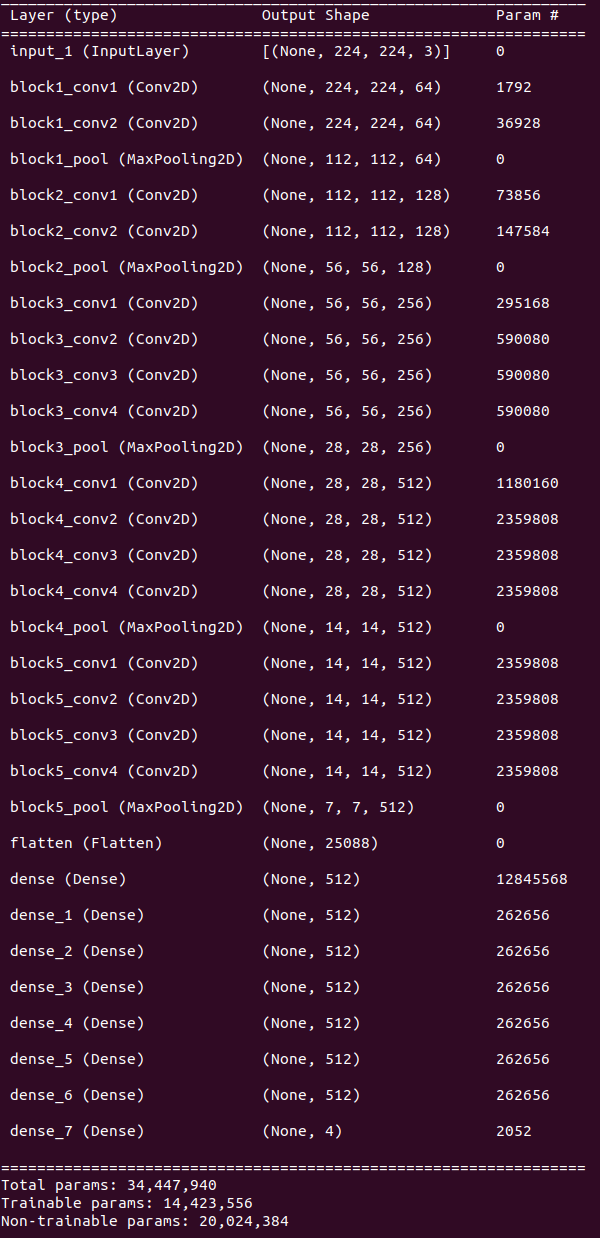
\includegraphics[scale=0.35]{Fig1}
  \caption{Costume dense layers}
  \label{Fig1}
\end{figure}

The custom fully connected layers start with the flatten layer, which flattens the output passed from the VGG19 convolution layer. Through flattening, we can have single-dimensional outputs instead of multi-dimensional outputs. 

Then there are seven dense layers with a rectified linear activation unit activation function. The reason for using the rectified linear activation unit as the activation function instead of the sigmoid or hyperbolic tangent function is that both the image and target coordinate output are normalized and distributed in the range between 0 and 1 so that the model can handle the prediction of input images with different image sizes, rather than a single fixed size. 

The last layer is a dense layer with the number of outputs to be predicted. The activation of this last dense layer is sigmoid, which is the one that performs better than other activation functions.


\section{Implementation details}
\label{detail}

\subsection{Dataset collection}
This project is implementing supervised learning which requires training images and target files.

\subsubsection{Image dataset}
The dataset of this project is a combination of the two versions of the CelebFaces Attributes Dataset. The two versions of the CelebA dataset have the same amount of images and duplicate CSV files. The main difference is that the first version of the image is the original copy which contains some parts of the body. The second version of the images is all cropped and aligned face images. 

The reason is that the bounding box target CSV file has the data based on the original images. On the other hand,  the target CSV files collect the aligned images' facial landmarks and facial attributes. Thus, two sets of images are required for this project to be done.

\subsubsection{Target CSV files}
There are four comma-separated values files in the dataset.
The first CSV file is about recommended training, validation, and testing split. Since the dataset gives the suggested data separation, this project will not implement k-fold validation or any other validation technique. 

\begin{figure}[!ht]
  \centering
  \begin{subfigure}{0.45\textwidth}
    \centering
    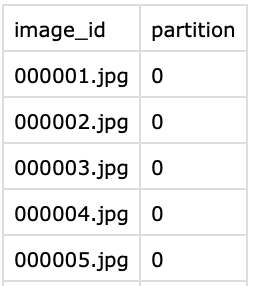
\includegraphics[scale=0.45]{Fig2}
    \caption{CSV Dataset Partition}
    \label{Fig2}
  \end{subfigure}
  \begin{subfigure}{0.45\textwidth}
    \centering
    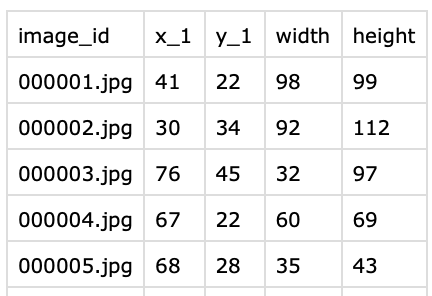
\includegraphics[scale=0.45]{Fig3}
    \caption{CSV BBox data}
    \label{Fig3}
  \end{subfigure}
  \begin{subfigure}{0.9\textwidth}
    \centering
    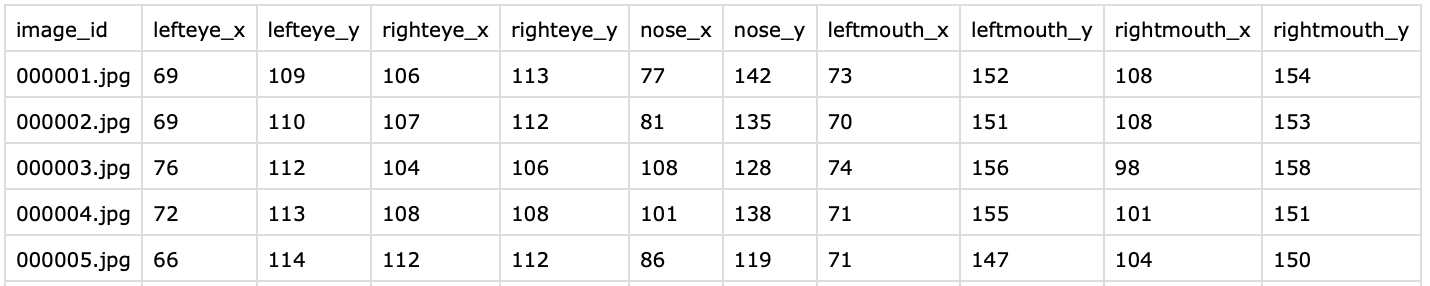
\includegraphics[scale=0.45]{Fig4}
    \caption{CSV Landmark data}
    \label{Fig4}
  \end{subfigure}
  \begin{subfigure}{0.9\textwidth}
    \centering
    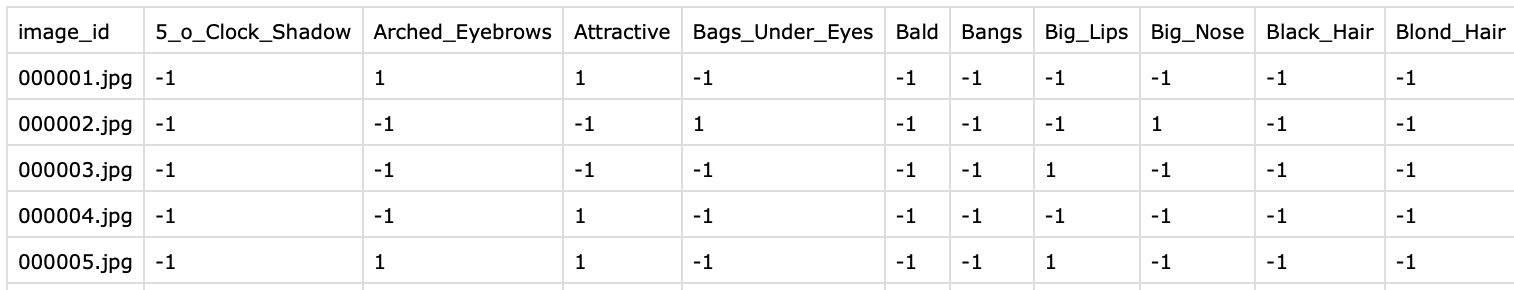
\includegraphics[scale=0.45]{Fig5}
    \caption{CSV Attributes data}
    \label{Fig5}
  \end{subfigure}
\end{figure}

The second CSV file is about the bounding box coordinates of the human face inside each image. There are two ways to define a bounding box position, two-point positioning and single-point with distance positioning. It is to use the coordinates of two points or one point and the height and width of the bounding box to locate the box position. This file stores the top left point coordinate and the width and height of the facial bounding box. 

The third CSV file is about the facial landmark coordinates of each image. The dataset only points out five of the facial landmarks: two eye pupils, tips of the nose, and two corners of the mouth. 

The fourth CSV file is about the existence of the forty facial attributes. Facial attributes include but are not limited to 5 o'clock Shadow, arched eybrows, attractiveness, bags under eyes, and much more. Each attribute's existence is marked as positive if it appears in the image and negative if the opposite. 

\subsection{Feature extraction}
The data features are being extracted by using image normalization and coordinate normalization. There are three applications of this transfer learning model for this particular problem which this project is trying to solve. And all three applications are having one common image dataset input as the training sample. But each of the three applications are having different supervisor data as the training targets. 

Image normalization is being practiced the easiest way, dividing each pixel by 255. This is because the maximum value a pixel can be, in the RGB colour model, is 255 which is colour white. Since the global maximum pixel value is known, it is not necessary to normalize it by other local maximum pixel values. 

\begin{figure}
  \centering
  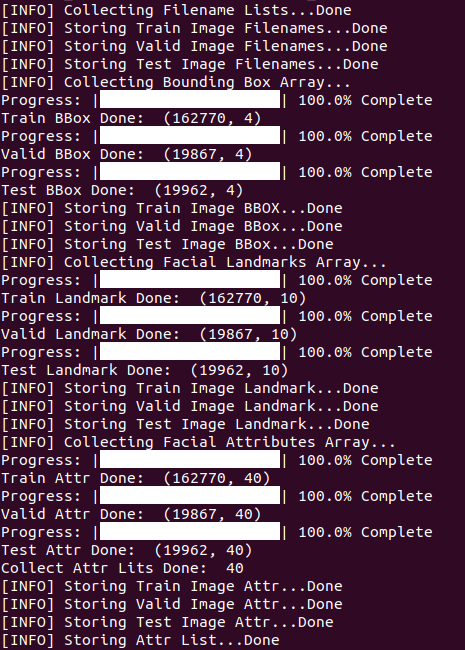
\includegraphics[scale=0.4]{Fig6}
  \caption{Data Preparation}
  \label{Fig6}
\end{figure}

There are two kinds of targeting data for the three applications, One is pixel coordinates or pixel location values for the prediction of the bounding box and facial landmarks. Another is binary true-or-false data and it is for the prediction of any facial attributes existence. The pixel coordinates need to be normalized by the dimension of the image. The width and height of the pictures are different, the size of each original picture is also different. This means that the normalization of each coordinate value must be carried out dynamically. On the other hand, the binary facial attributes do not require much modification. The only thing to do is to convert the default negative one as false into zero.

\subsection{Model construction}
The model of this project is a hybrid model constructed by using transfer learning. The convolutional part is from the VGG19 model and joins with the new custom fully connected layers. 

The VGG19 convolutional layers are sliced off the VGG19 model by not including the original fully connected top layers. The model weight is using the weights pre-trained in the ImageNet competition back in 2014. The weights were trained through 1.2 million images and 1000 classes of objects. Therefore, taking advantage of pre-trained weights can save a massive amount of training time. The default image input shape is 224x224 pixels with three color channels. Disable the model training for each layer so that the imagenet weights remain the original version, not modified after each additional training.

The custom fully connected layers have three groups of layers. The first is the input layer that takes the output from the VGG19 convolutional layers and flattens it. The second group of layers is hidden layers. The last layer is the output layer.

After testing and observing the change of training and validation loss of the model for varying numbers of hidden dense layers, setting the number of layers to be seven fully connected dense layers, the number of hidden nodes can also be concluded through the same procedures. The number of nodes is variants for different model applications. For the bounding box and facial attributes application, 512 hidden nodes in each hidden dense layer are suitable. In contrast, 4096 nodes in each hidden dense layer for the facial landmark application seem still not enough. As the number of nodes increases, the model performs better in learning accuracy and loss between prediction and the actual value until the curve peaks and drops. The node number and performance curve vary for different machines. Sometimes the machine crashes before the number of nodes reaches its best performance. 4096 is the number I got after hundreds of tests. The activation function uses the Rectified Linear Unit, which is due to the normalized data separation, all positive and between zero and one. Not using sigmoid as the hidden layer activation function is that sigmoid requires slightly more computation than ReLU. 

The output layer is one dense layer using the sigmoid activation function. The sigmoid curve is a continuous s-shape curve between zero and one. The targeting results of all three applications are also within the range of zero and one. Thus, sigmoid is a wise choice for this model. The number of output nodes varies for different model applications.

\begin{figure}
  \centering
  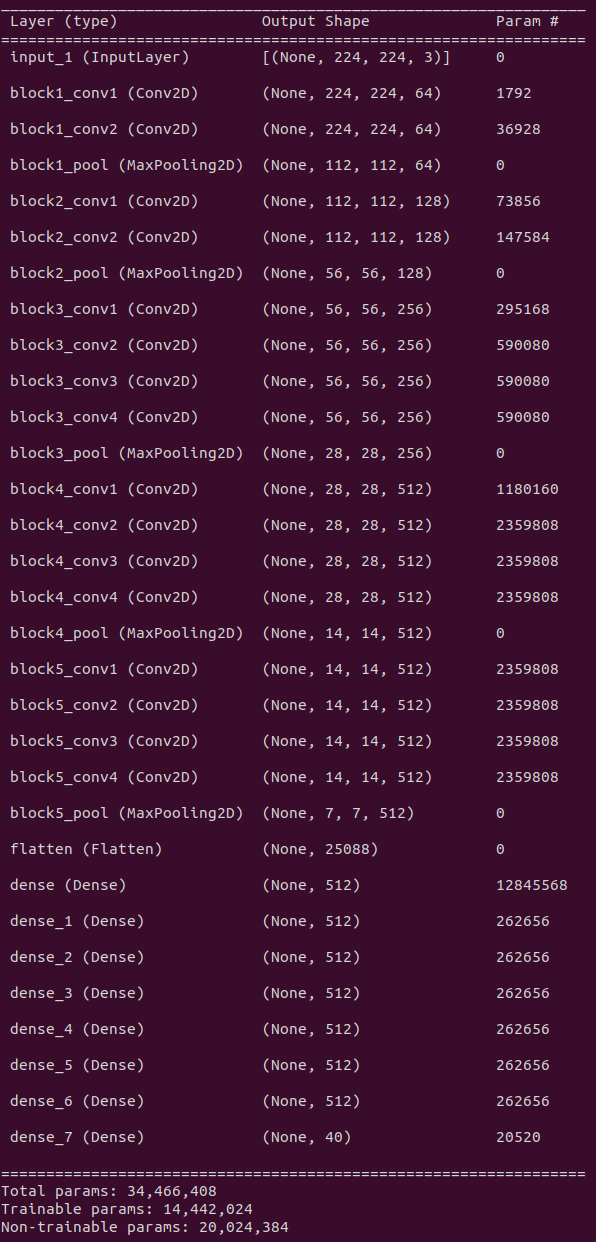
\includegraphics[scale=0.4]{Fig7}
  \caption{Model training summary}
  \label{Fig7}
\end{figure}

\subsection{Model compilation}
When compiling a model, the optimizer, the loss function, and the metrics to be monitored, there are three significant settings. The model uses adam as the optimization algorithm. Adma is a successor of stochastic gradient descent when training for deep learning models. The loss function and metrics of the model vary between different model applications. Mean square error loss is the most commonly used to predict the loss of non-binary results. Whereas, for binary targets, binary cross-entropy is a better choice. Similarly, for non-binary prediction, accuracy is the one used most. And there is also a corresponding one for binary prediction.

\subsection{Model training}
The image input for the VGG19 model is 224x224 pixels with three color channels by default. Use a multi-dimensional array to collect all the image data of a training batch. For that reason, the model needs to load and reshape the size of each image to 224x224 square with three color channels. Also, expand the dimension of the image by one so that all images can concatenate as one.   

The first thing to do is zip the input image and the input targets as one dataset for training, validation, and testing. For each training cycle, collect the image data for a batch size of 32 images. Smaller batch size can reduce the memory load and save the memory on information collection. The maximum number of training epochs is 100. A hundred epochs might be too much for a model with pre-trained weights, but it performs just fine with the help of early-stopping regularization. The early-stopping is to monitor the validation loss with three epochs of patients. It stops the model from training if it detects the validation loss not improving for three continuous epochs.  Another callback practiced in this model is using the checkpoint to save the best model weights if the current epoch of training has improved validation loss and not save if the validation loss gets worse or stays the same. 

\subsection{Drawbacks occurred while training}
Even though this model seems to handle and predict well on all three subdomain problems, there are still some disadvantages that are not solved.

\subsubsection{Landmark validation curve fluctuate}

\begin{figure}[ht]
  \centering
  \begin{subfigure}{0.45\textwidth}
    \centering
    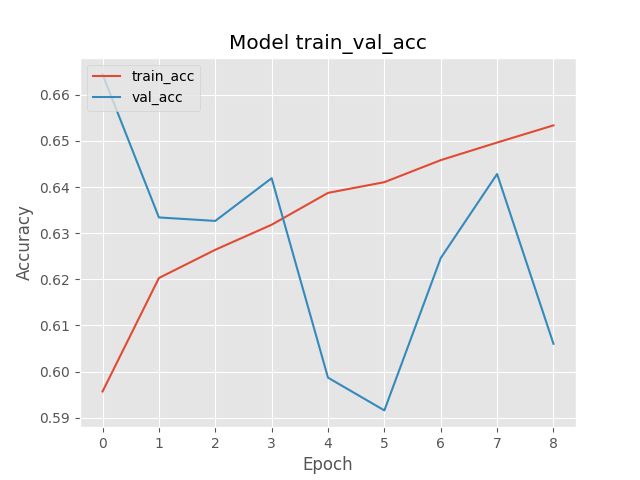
\includegraphics[width=\textwidth]{Fig8}
    \caption{Landmark training accuracy}
    \label{Fig8}
  \end{subfigure}
  \begin{subfigure}{0.45\textwidth}
    \centering
    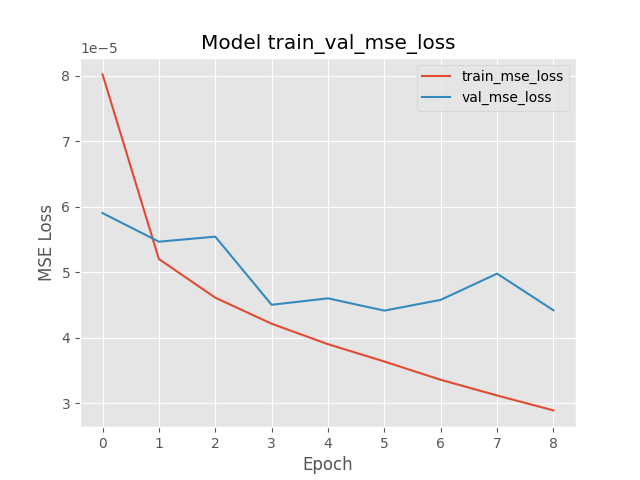
\includegraphics[width=\textwidth]{Fig9}
    \caption{Landmark training loss}
    \label{Fig9}
  \end{subfigure}
\end{figure}

In figures 9 and 10, the validation curve is fluctuating. The reason is not apparent at the time. Probably it is because of overfitting. However, both the training accuracy and loss curve is smooth and continuous making progress. Moreover, the losses of the model are minimal. The smaller the loss is better the predictions are. At this point, it can conclude that accuracy is not a good metric for evaluating landmark model performance. 

\subsubsection{Attributes accuracy}

\begin{figure}
  \centering
  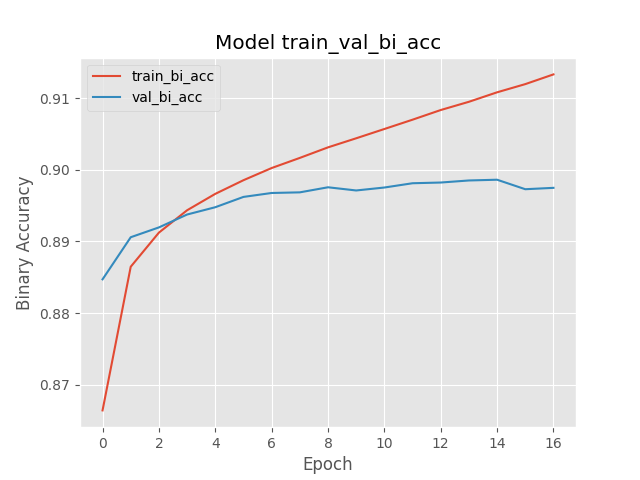
\includegraphics[scale=0.40]{Fig10}
  \caption{Attributes training accuracy}
  \label{Fig10}
\end{figure}

Although the training accuracy of the attributes reaches 91\%, as indicated in the figure 11, at the end of training cycles, it was approximately 99\% when training with one pair of coordinates instead of five pairs. After examining the training with different pairs of coordinates, it appears to be decreasing model accuracy as the number of pairs increases. Moreover, it occurs to be a negative effect between left and right eyes locations and the left and right mouse corner locations. Once these two coeffect coordinates are trained together, the model accuracy decreases significantly, down to 50\%. Probably it is due to the model complexity being low. 


\section{Results and evaluation}
\label{result}
The model is evaluated by using the testing dataset with the same loss function and metrics from the model compilation. The predicted result of each model application is reasonably acceptable and has space to improve as well. All model applications are having one significant issue that the model can only guarantee the prediction accuracy in testing the image from the default dataset, which that means for images not following the same feature distribution as the default dataset images, model prediction is not applicable. Taking facial landmarks prediction as an example, the model is trained with the image dataset with aligned images. The model prediction accuracy on testing images from the original image dataset will be ridiculously low. 

The proposed approach may not be significant compared with the state-of-the-art techniques listed in the third section. However, the approach is the beginning of practicing a single model with transfer learning on both image classification, image recognition, and image detection. 


\section{Conclusion and future work}
\label{future}
This paper proposed an approach to construct a single model by using transfer learning and applied this model with different types of image analysis. Even though the model prediction result of each application is not satisfying, the result is still reasonable and acceptable. The future work of this approach will be making it applicable for more applications and increasing the prediction accuracy at the same time.


\section*{References}

\small

[1] Zhuang, N., Yan, Y., Chen, S., Wang, H.,\ \&; Shen, C.\ (2018).\ Multi-label learning based deep transfer neural network for facial attribute classification. {\it Pattern Recognition}, {\bf80}, 225–240. doi: 10.1016/j.patcog.2018.03.018.

[2] Zheng, X., Guo, Y., Huang, H., Li, Y.,\ \&; He, R.\ (2020).\ A survey of deep facial attribute analysis. {\it International Journal of Computer Vision}, {\bf128}(8-9), 2002–2034. doi: 10.1007/s11263-020-01308-z.

[3] U. Mahbub, S. Sarkar and R. Chellappa, "Segment-Based Methods for Facial Attribute Detection from Partial Faces," in {\it IEEE Transactions on Affective Computing}, vol. {\bf11}, no. 4, pp. 601-613, 1 Oct.-Dec. 2020, doi: 10.1109/TAFFC.2018.2820048.

[4] S. Yang, P. Luo, C. C. Loy \& X. Tang, "Faceness-Net: Face Detection through Deep Facial Part Responses," in {\it IEEE Transactions on Pattern Analysis and Machine Intelligence}, vol. {\bf40}, no. 8, pp. 1845-1859, 1 Aug. 2018, doi: 10.1109/TPAMI.2017.2738644.

[5] Sun, Y., \&; Yu, J. (2018). General-to-specific learning for facial attribute classification in the wild. {\it Journal of Visual Communication and Image Representation}, {\bf56}, 83–91. doi: 10.1016/j.jvcir.2018.09.003. 

[6] L. Mao, Y. Yan, J. Xue \& H. Wang, "Deep Multi-task Multi-label CNN for Effective Facial Attribute Classification," in {\it IEEE Transactions on Affective Computing}, doi: 10.1109/TAFFC.2020.2969189.

[7] J. Li, F. Zhao, J. Feng, S. Roy, S. Yan \& T. Sim, "Landmark Free Face Attribute Prediction," in {\it IEEE Transactions on Image Processing}, vol. {\bf27}, no. 9, pp. 4651-4662, Sept. 2018, doi: 10.1109/TIP.2018.2839521.

[8] A. F. Abate, P. Barra, S. Barra, C. Molinari, M. Nappi \& F. Narducci, "Clustering Facial Attributes: Narrowing the Path From Soft to Hard Biometrics," in {\it IEEE Access}, vol. {\bf8}, pp. 9037-9045, 2020, doi: 10.1109/ACCESS.2019.2962010.

[9] M. Sadiq, D. Shi, M. Guo \& X. Cheng, "Facial Landmark Detection via Attention-Adaptive Deep Network," in {\it IEEE Access}, vol. {\bf7}, pp. 181041-181050, 2019, doi: 10.1109/ACCESS.2019.2955156.

[10] N. Zhu, Z. Yu \& C. Kou, "A New Deep Neural Architecture Search Pipeline for Face Recognition," in {\it IEEE Access}, vol. {\bf8}, pp. 91303-91310, 2020, doi: 10.1109/ACCESS.2020.2994207.

[11] Chen, P., Hang, H., Chan, S., \& Lin, J. (2020). DSNet: An efficient CNN for road scene segmentation. {\it APSIPA Transactions on Signal and Information Processing}, {\bf9}, E27. doi:10.1017/ATSIP.2020.25

\end{document}
